\section{Auto Model Selection}
\label{sec:autoModelSelection}

Our first approach is to evaluate a lot of models against a reference dataset and record \(RMSSE\), the time it took to fit \(t_{fit}\) and the time it took to predict the forecast \(t_{predict}\) given a model and its parameters. Out of this collected data we elect the best model for each timeseries in the dataset. Given this information, we then try to setup a multi-class classification learning task. The timeseries data is \(X\) and the best model is our target variable \(y\). The hypothesis is that the timeseries themselves contain enough information to predict the best model.

In each experiment we restrict ourselves to a single but large dataset and a fixed forecast horizon.

\subsection{Datasets}

We used two datasets to run two experiments. The first dataset is the \textbf{Web Traffic Timeseries Forecasting} competition \cite{web-traffic-competition} data. The dataset consists of roughly 145,000 timeseries representing traffic to a Wikipedia article page. The resolution of the data is daily and ranges from 2015-07-01 to 2017-09-10 which is 803 data points. The task is to create a forecast from 2017-09-13 to 2017-11-13 which is a 65-day horizon. There are about 8\% of missing values in this dataset, which is not making it trivial. The page names can be grouped by language and user agent. A distribution of traffic to languages over time is shown in figure \ref{fig:wiki_lang_distribution}.


\begin{figure*}
\centerline{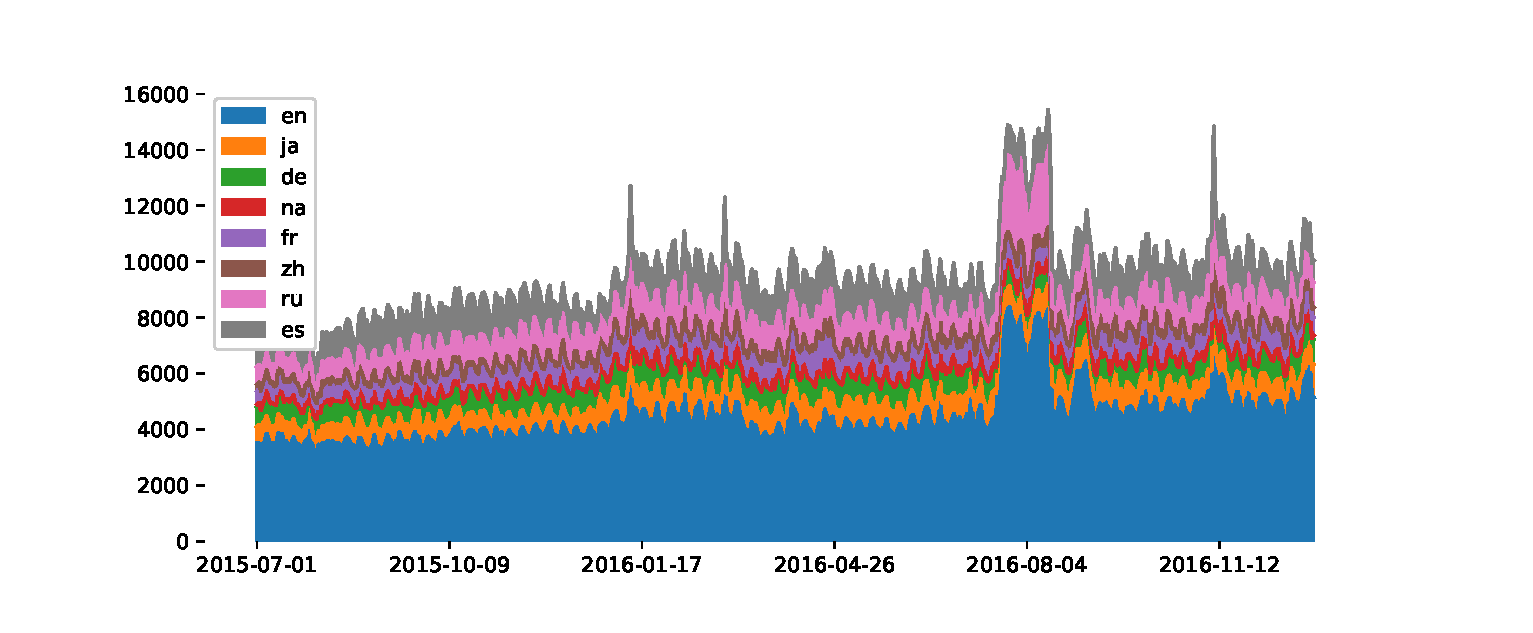
\includegraphics[scale=.6]{Figures/wiki_lang_distribution.eps}}
\caption{The Wiki Traffic dataset contains around 145,000 timeseries. This chart shows them summed and grouped by language. We find that English pages are the most common in the dataset. We can also clearly see a strong weekly seasonal pattern and a significant increase in traffic around 2016-08-04.}
\label{fig:wiki_lang_distribution}
\end{figure*}

The second dataset is the \textbf{M5 Forecasting Accuracy} competition \cite{M5} data. It consists of roughly 30,500 timeseries representing article sales. The resolution of the data is daily and ranges from 2011-01-29 to 2016-06-19 which is 1941 data points. The task is to create a 28-day forecast for each article. Many articles in this dataset went out of sale, thus we should probably predict zero for timeseries which have been sold zero times towards the end of the timeseries. A distribution of sales of product categories is shown in figure \ref{fig:m5_cat_distribution}.


\begin{figure*}
\centerline{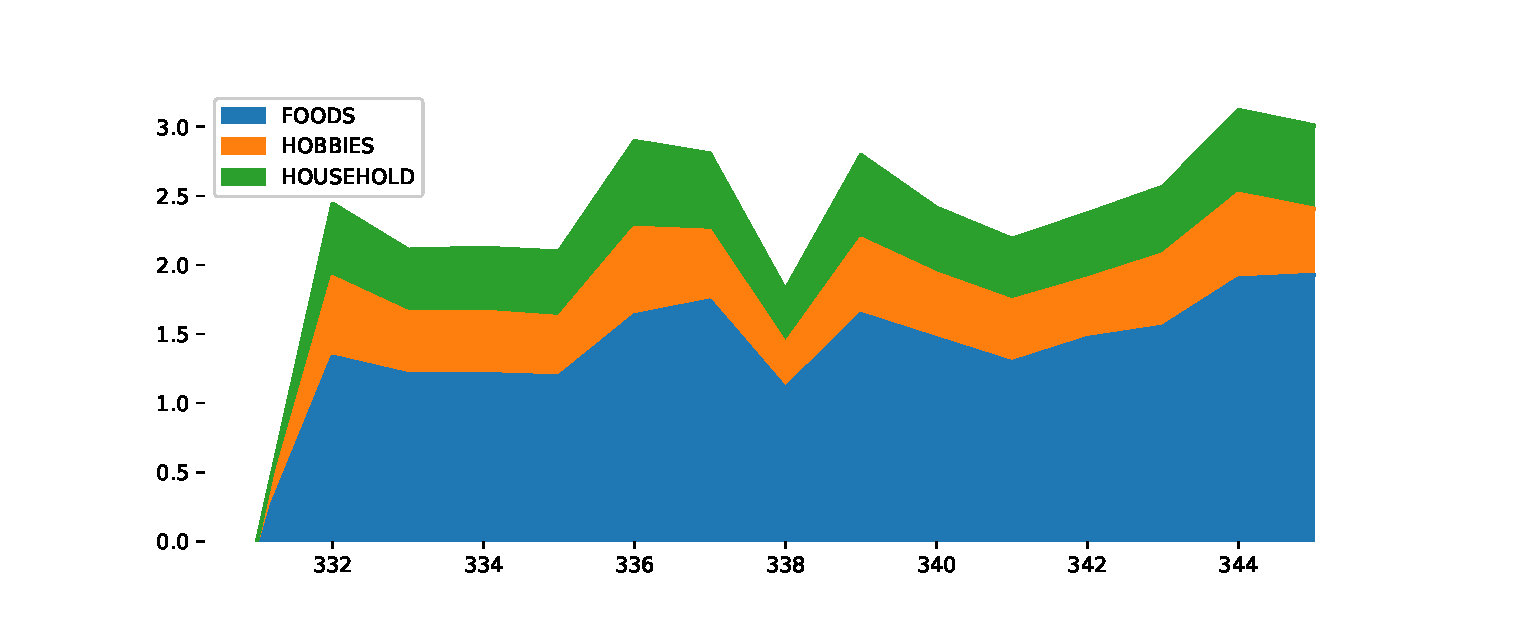
\includegraphics[scale=.6]{Figures/m5_cat_distribution.eps}}
\caption{The M5 competition dataset contains around 30,500 timeseries. This chart shows them summed and grouped by item category. We find that there is a strong weekly seasonal pattern and a general upwards trend. We also see a yearly pattern that shows food and hobby items are not being sold on a particular day. This happens to be December 25, Christmas.}
\label{fig:m5_cat_distribution}
\end{figure*}


\subsection{Evaluating Models}

We start with a large number of different models and implement each and wrap it in a common API that allows us to fit a timeseries and create a forecast. We based our implementation on sktime \cite{sktime} as they have implemented a common API for many models already. Some needed a few tweaks (Prophet) and others are regression-based pipelines that needed to be assembled. For more details which 34 models were used refer to the model overview. For each model we defined a parameter grid based on the available parameters of the model and a sensible impression that the values can make sense. We then exploded the parameter grids into all its combinations and ended up with a model of of 1451. A distribution of combinations by model type can be seen in figure \ref{fig:model_numbers}.

\begin{figure*}
\centerline{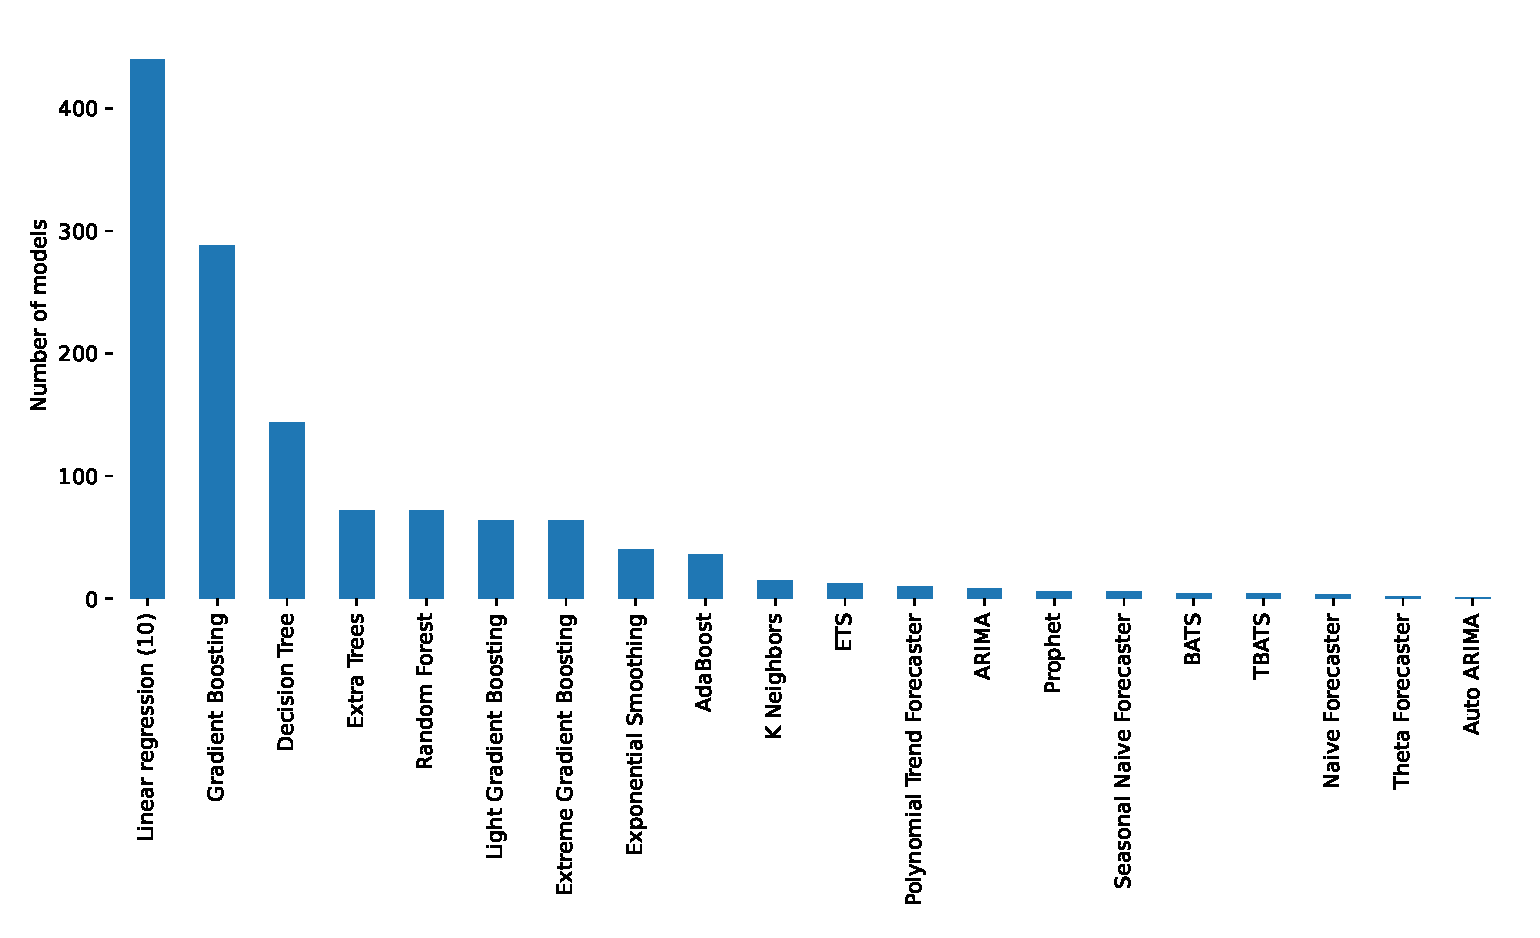
\includegraphics[scale=.6]{Figures/model_numbers.eps}}
\caption{Distribution of the hyper-parameter combinations by model. We aggregated the 10 linear regression-based models.}
\label{fig:model_numbers}
\end{figure*}


Additionally, we wanted to be able to compare models with different error metrics such as RMSSE, MAPE and SMAPE. Hence, we implemented each metric and wrapped in a common API as well. Each produced forecast error would then be computed by each metric formula.

Evaluating 1451 different models against 145,000 is not feasible. Thus, we iteratively eliminated models by selecting a small sample of timeseries and evaluating all models against it. The first ones to be removed are the models that take too long to fit. We set the threshold at 10 seconds initially. In our setup we used a Macbook Pro with a 2.6 GHz 6-Core Intel Core i7 processor. This meant the following models were removed from the list with their average fit and predict times combined: TBATS (21.s) and BATS (11.4s). For XGBoost we had to remove the n\textunderscore estimators parameter value of 300, and for LightGBM we had to remove the num\textunderscore leaves value 8 and n\textunderscore estimators value 300. We then continued pruning the models further by removing the ones with high RMSSE values and at the same time increasing the sample size as fewer models were contained in the list. 

To create labels for a classifier to learn we had to elect the best model per timeseries, for which it is important to have a large sample size of timeseries and optimally as few unique labels as possible. Unfortunately, we did not converge on a few models but had several hundreds of models that were at least once the best performing model for a single timeseries. We need to reduce the number of models. We could have aggregated by model type and ignore parameters. This however would not give good results when applying this model to a new timeseries as we either end up with an un-tuned model or we end up tuning it, which is something we wanted to avoid for time and cost reasons. We also did not want to compare models on an average error metric as they each excel at different timeseries, once they perform outstanding, and other times they produce very high error forecasts. So, we decided for each timeseries to sort the models by their RMSSE score and take the 10\textsuperscript{th} percentile best ones and increment their select score. Doing this for all timeseries gave us a score per model of how many times it was under the best performing models.

We still had models that excelled at exactly one timeseries. This leads to a problem that we cannot include models that have one attached timeseries and expect that a classifier would learn that classification. We need to reach a minimum sample size per model. Thus, we drastically reduced the number of models until we ended up with the 7 best performing models over all. The final models were AdaBoost, Decision Tree with Conditional Deseasonalize \& Detrending, Exponential Smoothing (Holt-Winters) and sNa\"ive. With their parameter combinations we had come down to 9 models. The models also nicely distributed so we had a balanced dataset. We chose the best model per timeseries to avoid having a multilabel problem besides our multiclass problem.


\subsection{Classifying Timeseries}

The next step was to build a classifier with the labels that we generated by evaluating the models. There are several methods that we tried.

\textbf{Feature Extraction:} The first method was to extract statistical features from the timeseries and use this feature vector as input to a traditional classifier. To improve our chances of finding relevant features we tried to extract as many features as possible per timeseries. The authors of tsfresh \cite{tsfresh} have implemented a vast amount of feature calculators and many possible combinations thereof. They range from mean, min, max, autocorrelation, count below x, fast fourier transform, quantiles and so forth. A complete extraction results in 4,722 features many of which are the features but with different arguments such as threshold. Some feature extractors are a bit slow however and would make this unpractical for us, since we want to classify a timeseries quickly. Thus, the reduce set of minimal feature extractors is 54. 

% TODO feature importances

We then evaluated a series of classifiers, namely decision tree, random forest and SVM \cite{SVM} to fit this data. The cross-validation precision, recall and F1 scores were unfortunately unusable. To make this Auto Model Selection approach work we would need to achieve a high precision of 80\% to 90\%. We tried to ignore the model parameters and try to classify based on model type. Yes, we said that this would not be a useful use case, but it would be interesting if there is a way to simplify the classification problem to get a relevant accuracy out of it. The result is shown in figure \ref{fig:classifier_metrics}.

\begin{figure*}
    \begin{verbatim}
                       precision    recall  f1-score   support
    
      ada_cds_dt       0.00      0.00      0.00        36
       dt_cds_dt       0.00      0.00      0.00        40
      exp_smooth       0.33      0.35      0.34        82
          snaive       0.37      0.64      0.47        92
    \end{verbatim}
    \caption{The best performing classifier was SVM. However, it only learned to separate between Exponential Smoothing and sNa\"ive. The AdaBoost and Decision Tree methods were never recognized.}
    \label{fig:classifier_metrics}
\end{figure*}

\textbf{ROCKET:} Another method to classify timeseries data is ROCKET (\textbf{R}and\textbf{O}m \textbf{C}onvolutional \textbf{KE}rnel \textbf{T}ransform) \cite{ROCKET}. ROCKET can achieve state-of-the-art classification accuracy while using a fraction of the time required by other recent scalable methods. It transforms timeseries using random convolutional kernels into features. To generate the random kernels ROCKET chooses random values for length, weights, bias, dilation and padding. The transformed features can be used to train a linear classifier. The authors recommend a ridge classifier. With ROCKET we achieved a similar result that we had with standard Feature Extraction and training a tree based classifier. We reached a precision of 32\%. We find that even by changing the method, we cannot gain better classification performance. We can say however that the ROCKET method is much faster than extracting all 4,722 features and run a tree classifier. However, if we only extract the features that are actually important, ROCKET loses out on CPU time compared to the previous method.


\textbf{Others:} We also tried other timeseries classification methods such as MrSEQL \cite{MRSEQL}, Random Interval Spectral Forest (RISE) \cite{RISE} and a k-Neighbors based time series classifier. With MrSEQL we reached the same score 32\% as with ROCKET. With Random Interval Spectral Forest and k-neighbors we both got 28\% for precision.

\subsection{Results}

We find that evaluating a large range of models and their parameters against a large timeseries dataset can be tedious. The space for optimization of this process is big. PyCaret \cite{PyCaret} is planning to ship a timeseries module in the future which could potentially be used to get faster results. However, PyCaret will only do it for one timeseries. We would still need to create an optimized evaluation execution over many timeseries.
The classification of timeseries out of one dataset has been proofed complex. The datasets we used contained all in a sense similar timeseries. This was intentionally chosen as with this approach we wanted to be able to find the best model per timeseries, not per dataset. Future research on experiment setup and tweaks to this approach might lead to better results than what we got. For us we concluded that this approach is one level too deep. Instead, we should look at the learning task parameters and the basic characteristics of the timeseries, which is a level higher, to do the model selection. This second approach is explained in the next section.
